\section{ECFactory\-Base Class Reference}
\label{classECFactoryBase}\index{ECFactoryBase@{ECFactoryBase}}
Inheritance diagram for ECFactory\-Base::\begin{figure}[H]
\begin{center}
\leavevmode
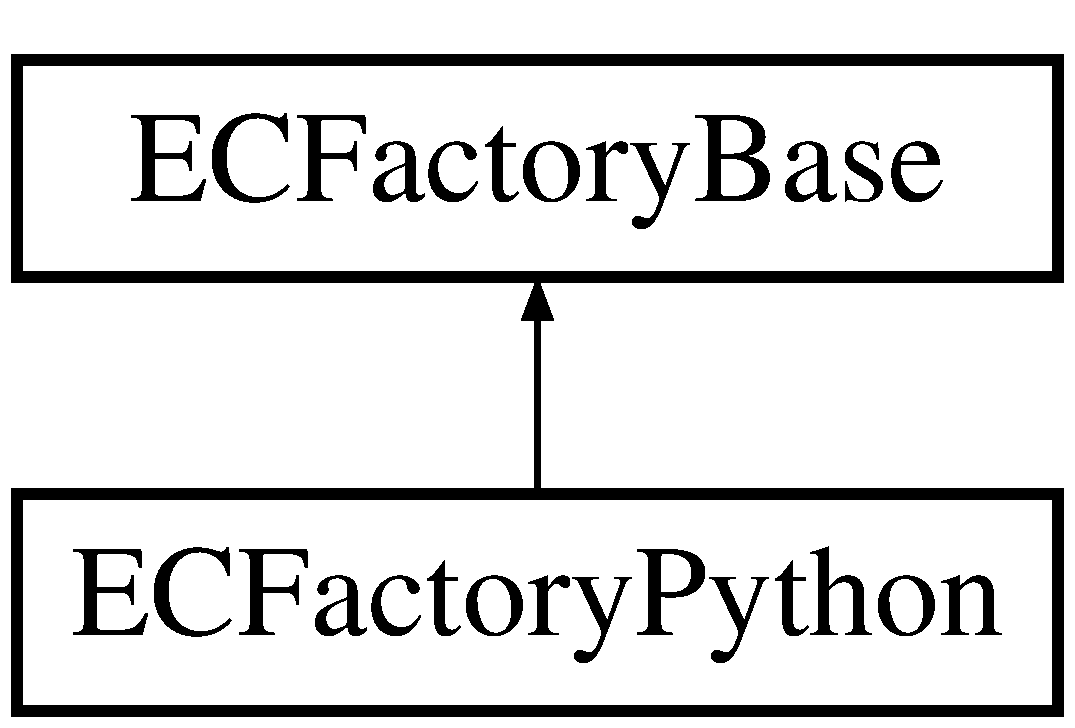
\includegraphics[height=2cm]{classECFactoryBase}
\end{center}
\end{figure}
\subsection*{Public Member Functions}
\begin{CompactItemize}
\item 
{\bf \_\-\_\-init\_\-\_\-} ()
\item 
{\bf name} ()
\item 
{\bf create} ()
\item 
{\bf destroy} (comp)
\end{CompactItemize}


\subsection{Member Function Documentation}
\index{ECFactoryBase@{ECFactory\-Base}!__init__@{\_\-\_\-init\_\-\_\-}}
\index{__init__@{\_\-\_\-init\_\-\_\-}!ECFactoryBase@{ECFactory\-Base}}
\subsubsection{\setlength{\rightskip}{0pt plus 5cm}ECFactory\-Base::\_\-\_\-init\_\-\_\- ()}\label{classECFactoryBase_ECFactoryPythona5}


\index{ECFactoryBase@{ECFactory\-Base}!create@{create}}
\index{create@{create}!ECFactoryBase@{ECFactory\-Base}}
\subsubsection{\setlength{\rightskip}{0pt plus 5cm}ECFactory\-Base::create ()}\label{classECFactoryBase_ECFactoryBasea2}




Reimplemented in {\bf ECFactory\-Python} {\rm (p.\,\pageref{classECFactoryPython_ECFactoryPythona3})}.\index{ECFactoryBase@{ECFactory\-Base}!destroy@{destroy}}
\index{destroy@{destroy}!ECFactoryBase@{ECFactory\-Base}}
\subsubsection{\setlength{\rightskip}{0pt plus 5cm}ECFactory\-Base::destroy (comp)}\label{classECFactoryBase_ECFactoryPythona6}


\index{ECFactoryBase@{ECFactory\-Base}!name@{name}}
\index{name@{name}!ECFactoryBase@{ECFactory\-Base}}
\subsubsection{\setlength{\rightskip}{0pt plus 5cm}ECFactory\-Base::name ()}\label{classECFactoryBase_ECFactoryBasea1}




Reimplemented in {\bf ECFactory\-Python} {\rm (p.\,\pageref{classECFactoryPython_ECFactoryPythona2})}.

The documentation for this class was generated from the following file:\begin{CompactItemize}
\item 
{\bf ECFactory.py}\end{CompactItemize}
